

\tikzset{every picture/.style={line width=0.75pt}} %set default line width to 0.75pt        

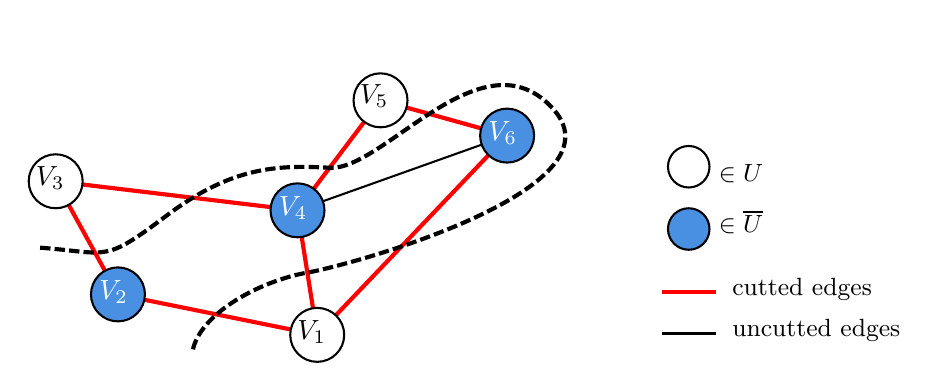
\begin{tikzpicture}[x=0.75pt,y=0.75pt,yscale=-1,xscale=1]
%uncomment if require: \path (0,159); %set diagram left start at 0, and has height of 159

%Straight Lines [id:da11964796995332005] 
\draw    (158.5,73.5) -- (259.5,37.5) ;
%Straight Lines [id:da15972910359553594] 
\draw [color={rgb, 255:red, 255; green, 0; blue, 0 }  ,draw opacity=1 ][line width=1.5]    (158.5,73.5) -- (168,133.5) ;
%Straight Lines [id:da2798044521653187] 
\draw [color={rgb, 255:red, 255; green, 0; blue, 0 }  ,draw opacity=1 ][line width=1.5]    (259.5,37.5) -- (198.5,20.5) ;
%Straight Lines [id:da7169631782552711] 
\draw [color={rgb, 255:red, 255; green, 0; blue, 0 }  ,draw opacity=1 ][line width=1.5]    (158.5,73.5) -- (198.5,20.5) ;
%Straight Lines [id:da026668841375865227] 
\draw [color={rgb, 255:red, 255; green, 0; blue, 0 }  ,draw opacity=1 ][line width=1.5]    (168,133.5) -- (259.5,37.5) ;
%Straight Lines [id:da10247267579193942] 
\draw [color={rgb, 255:red, 255; green, 0; blue, 0 }  ,draw opacity=1 ][line width=1.5]    (158.5,73.5) -- (42,59.5) ;
%Straight Lines [id:da6325731661518962] 
\draw [color={rgb, 255:red, 255; green, 0; blue, 0 }  ,draw opacity=1 ][line width=1.5]    (168,133.5) -- (72,114) ;
%Straight Lines [id:da6714305559976217] 
\draw [color={rgb, 255:red, 255; green, 0; blue, 0 }  ,draw opacity=1 ][line width=1.5]    (72,114) -- (42,59.5) ;
%Shape: Ellipse [id:dp9445310521915122] 
\draw  [fill={rgb, 255:red, 74; green, 144; blue, 226 }  ,fill opacity=1 ] (246.5,37.5) .. controls (246.5,30.32) and (252.32,24.5) .. (259.5,24.5) .. controls (266.68,24.5) and (272.5,30.32) .. (272.5,37.5) .. controls (272.5,44.68) and (266.68,50.5) .. (259.5,50.5) .. controls (252.32,50.5) and (246.5,44.68) .. (246.5,37.5) -- cycle ;
%Shape: Ellipse [id:dp5491993786197626] 
\draw  [fill={rgb, 255:red, 255; green, 255; blue, 255 }  ,fill opacity=1 ] (29,59.5) .. controls (29,52.32) and (34.82,46.5) .. (42,46.5) .. controls (49.18,46.5) and (55,52.32) .. (55,59.5) .. controls (55,66.68) and (49.18,72.5) .. (42,72.5) .. controls (34.82,72.5) and (29,66.68) .. (29,59.5) -- cycle ;
%Curve Lines [id:da8424711661169174] 
\draw [line width=1.5]  [dash pattern={on 3.75pt off 1.5pt}]  (34.5,91.5) .. controls (68,94) and (64.56,99.23) .. (95.5,76) .. controls (126.44,52.77) and (148,51.5) .. (174,53) .. controls (200,54.5) and (248,-13.5) .. (281.92,24.92) .. controls (315.83,63.33) and (185.58,99.58) .. (163.25,103.5) .. controls (140.92,107.42) and (111.42,122.92) .. (107.92,141.42) ;
%Shape: Ellipse [id:dp8814510692429732] 
\draw  [fill={rgb, 255:red, 255; green, 255; blue, 255 }  ,fill opacity=1 ] (337,52.5) .. controls (337,46.98) and (341.48,42.5) .. (347,42.5) .. controls (352.52,42.5) and (357,46.98) .. (357,52.5) .. controls (357,58.02) and (352.52,62.5) .. (347,62.5) .. controls (341.48,62.5) and (337,58.02) .. (337,52.5) -- cycle ;
%Shape: Ellipse [id:dp47339460639922903] 
\draw  [color={rgb, 255:red, 0; green, 0; blue, 0 }  ,draw opacity=1 ][fill={rgb, 255:red, 74; green, 144; blue, 226 }  ,fill opacity=1 ] (337,82.5) .. controls (337,76.98) and (341.48,72.5) .. (347,72.5) .. controls (352.52,72.5) and (357,76.98) .. (357,82.5) .. controls (357,88.02) and (352.52,92.5) .. (347,92.5) .. controls (341.48,92.5) and (337,88.02) .. (337,82.5) -- cycle ;
%Straight Lines [id:da23538055750108888] 
\draw [color={rgb, 255:red, 255; green, 0; blue, 0 }  ,draw opacity=1 ][line width=1.5]    (359.92,113) -- (334,113) ;
\draw [color={rgb, 255:red, 0; green, 0; blue, 0 }  ,draw opacity=1 ][line width=1.0]    (359.92,133) -- (334,133) ;
%Shape: Ellipse [id:dp4410323283239628] 
\draw  [fill={rgb, 255:red, 255; green, 255; blue, 255 }  ,fill opacity=1 ] (185.5,20.5) .. controls (185.5,13.32) and (191.32,7.5) .. (198.5,7.5) .. controls (205.68,7.5) and (211.5,13.32) .. (211.5,20.5) .. controls (211.5,27.68) and (205.68,33.5) .. (198.5,33.5) .. controls (191.32,33.5) and (185.5,27.68) .. (185.5,20.5) -- cycle ;
%Shape: Ellipse [id:dp23920294173784062] 
\draw  [fill={rgb, 255:red, 74; green, 144; blue, 226 }  ,fill opacity=1 ] (145.5,73.5) .. controls (145.5,66.32) and (151.32,60.5) .. (158.5,60.5) .. controls (165.68,60.5) and (171.5,66.32) .. (171.5,73.5) .. controls (171.5,80.68) and (165.68,86.5) .. (158.5,86.5) .. controls (151.32,86.5) and (145.5,80.68) .. (145.5,73.5) -- cycle ;
%Shape: Ellipse [id:dp6646352421974419] 
\draw  [fill={rgb, 255:red, 255; green, 255; blue, 255 }  ,fill opacity=1 ] (155,133.5) .. controls (155,126.32) and (160.82,120.5) .. (168,120.5) .. controls (175.18,120.5) and (181,126.32) .. (181,133.5) .. controls (181,140.68) and (175.18,146.5) .. (168,146.5) .. controls (160.82,146.5) and (155,140.68) .. (155,133.5) -- cycle ;
%Shape: Ellipse [id:dp5494896623298657] 
\draw  [fill={rgb, 255:red, 74; green, 144; blue, 226 }  ,fill opacity=1 ] (59,114) .. controls (59,106.82) and (64.82,101) .. (72,101) .. controls (79.18,101) and (85,106.82) .. (85,114) .. controls (85,121.18) and (79.18,127) .. (72,127) .. controls (64.82,127) and (59,121.18) .. (59,114) -- cycle ;

% Text Node
\draw (31,50.9) node [anchor=north west][inner sep=0.75pt]  [font=\normalsize]  {$V_{3}$};
% Text Node
\draw (360,50) node [anchor=north west][inner sep=0.75pt]  [font=\small]  {$\in U$};
% Text Node
\draw (360,72) node [anchor=north west][inner sep=0.75pt]  [font=\small]  {$\in \overline{U}$};
% Text Node
\draw (366.5,104.5) node [anchor=north west][inner sep=0.75pt]  [font=\small] [align=left] {cutted edges};
\draw (366.5,124.5) node [anchor=north west][inner sep=0.75pt]  [font=\small] [align=left] {uncutted edges};
% Text Node
\draw (187,11.4) node [anchor=north west][inner sep=0.75pt]  [font=\normalsize]  {$V_{5}$};
% Text Node
\draw (249,29.4) node [anchor=north west][inner sep=0.75pt]  [font=\normalsize,color={rgb, 255:red, 255; green, 255; blue, 255 }  ,opacity=1 ]  {$V_{6}$};
% Text Node
\draw (148,65.4) node [anchor=north west][inner sep=0.75pt]  [font=\normalsize,color={rgb, 255:red, 255; green, 255; blue, 255 }  ,opacity=1 ]  {$V_{4}$};
% Text Node
\draw (157,124.9) node [anchor=north west][inner sep=0.75pt]  [font=\normalsize]  {$V_{1}$};
% Text Node
\draw (61.5,105.9) node [anchor=north west][inner sep=0.75pt]  [font=\normalsize,color={rgb, 255:red, 255; green, 255; blue, 255 }  ,opacity=1 ]  {$V_{2}$};


\end{tikzpicture}
